\scanpage{89}
% archive foliation: 88
\unsure{Transitivité} :
\deleted{[ N.B. il suffit de le vérifier pour des ouverts \deleted{\unsure{aff.}} affines quasi-compacts \inserted{$U^\alpha$} recouvrant $X$, et pour tt $U^\alpha$ \unsure{trouver} un \uline{recouvrement} de $U^\alpha$ par des parties \deleted{constructibles} \inserted{loc. fermées} $U_i^\alpha$, tels que $f\,|\,|U_i^\alpha|$ soit \deleted{\unsure{aff.}} morphisme \ldots}
\margin{$\unsure{\varphi}$}
\margin{\uline{Proposition}}

On appelle \uline{ensemble} \deleted{\unsure{algébrique}}\deleted{\illegible{1}} \uline{schématique} un \deleted{préschéma}, \inserted{préschéma quasi-séparé quasi-compact,} considéré comme objet d'une catégorie dont les morphismes sont les applications constructibles.

\diagram{\begin{tikzcd}[ampersand replacement=\&,column sep=small]
(\mathrm{Sch}\ \deleted{\unsure{\text{réd}}}) \arrow[r] \arrow[rr,bend right=32,"{\deleted{\text{fidèle}}}"'] \arrow[rrr,bend right=48,"{\deleted{\text{fidèle}}}"'] \&
(\mathrm{Sch}) \arrow[r,"{\unsure{\text{n'd}}\ \deleted{\text{fidèle}}}"'] \arrow[rr,bend right=23,"{\deleted{\unsure{\text{fidèle}}}}"'] \&
(\mathrm{ens\ Sch}) \arrow[r,"{\text{fidèle}}"'] \&
(\mathrm{Sch.\ atomes}) \arrow[r,"{\text{pl.\ fid.}}"'] \&
\underline{\mathrm{Hom}}((\mathrm{corps}),\mathrm{Ens})
\end{tikzcd}}

\margin{\figure{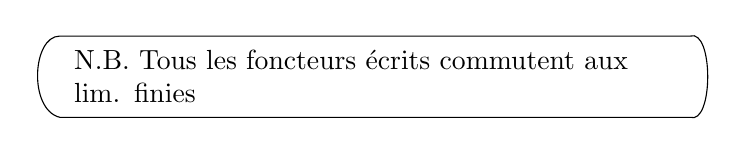
\begin{tikzpicture}
\node[anchor=west,text width=.63\linewidth,inner sep=5pt] (nb) at (0,0) {N.B. \unsure{Tous} les foncteurs écrits commutent aux \unsure{lim.} finies};
\draw (nb.north west) .. controls +(-.35,0) and +(-.4,.1) .. (nb.south west) -- (nb.south east) .. controls +(.3,-.1) and +(.3,.1) .. (nb.north east) -- cycle;
\end{tikzpicture}}}

On s'intéresse \unsure{donc} aux notions sur les ens. schématiques, qui sont invariantes par isom. d'ens schématiques (i.e. isom. constructibles).

Notons $\unsure{\mathfrak S|\mathsection}$ \unsure{comme} \unsure{l.c.q.|l.c.p.}

\diagram{\begin{tikzcd}[ampersand replacement=\&]
X\arrow[r]\&Y\\
X_i\&Y_i\\
X'_j\&\\
X_i\cap X'_j\arrow[r]\&Y_{ij}
\end{tikzcd}}

\uline{Lemme} Soit $X$ préschéma quasi-compact quasi-séparé. \deleted{Alors il existe une} $(Z_i)$ une famille \unsure{quelconque} de parties constructibles recouvrant $X$. Alors il existe une partition de $X$ en des parties loc. fermées constructibles affines, \unsure{plus fine qu'un recouvrement de $X$ par des ens. constructibles}.

\uline{Proposition} Supposons $X$ quasi-séparé et quasi-compact, $f:|X|\longrightarrow|Y|$ donné. Conditions équivalentes

\unsure{a)|i)} $f$ est constructible

\unsure{iii)|ii)} $\exists$ une partition \inserted{finie} de $X$ en des parties \uline{loc. fermées constructibles} $Z_i$, \inserted{\uline{affines}}, telles que $f\,|\,|Z_i|$ soit morphisme

\deleted{\unsure{iii)} Il existe une suite croissante d'ouverts quasi-compacts $U_i$ couvrant $X$, telle que $f\,|\,|U_i-U_{i-1}|$ soit \unsure{morphisme}.}
\figure{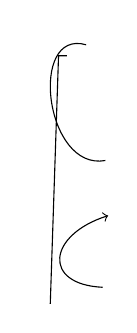
\begin{tikzpicture}[x=.7cm,y=.7cm]
\draw (0,4.5)--(-.15,4.5)--(-.3,0);
\draw (.35,4.7) .. controls (-.7,5) and (-.4,2.4) .. (.7,2.6);
\draw[->] (.65,.3) .. controls (-.45,.35) and (-.35,1.25) .. (.75,1.6);
\end{tikzpicture}}
% The blue reversed typewriting is show-through; its printed face is on scan 90.
